\chapter{Discussion}
Please tell more about conclusion and how to the next work of this study.

\section{Annisa Fathoroni/1164067}
\subsection{Teori}
Penjelasan Tugas Harian 11 ( No 1-8 ).
\begin{enumerate}
\item Mengapa file suara harus dilakukan MFCC, dilengkapi dengan ilustrasi atau gambar.

Mel Frequency Cepstral Coefficients (MFCC) merupakan koefisien yang merepresentasikan audio. Sehingga diharuskannya melakukan MFCC kepada objek suara atau audio agar suara dapat berubah atau diubah ke dalam bentuk data matrix dimana telah dilakukan ekstraksi oleh MFCC kemudian direalisasikan sebagai data matrix.

\begin{itemize}
\item Ilustrasi Gambar:

\begin{figure}[!hbtp]
\centering
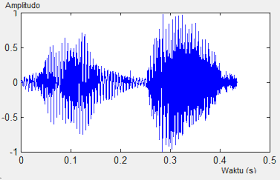
\includegraphics[scale=0.7]{figures/Chapter6AnnisaFathoroni1.png}
\caption{MFCC - Annisa Fathoroni}
\label{MFCC - Annisa Fathoroni}
\end{figure}

\end{itemize}

\item Konsep dasar Neural Network, dilengkapi dengan ilustrasi atau gambar.

Neural Network merupakan replika dari sistem syaraf yang terdapat pada sistem otak manu- sia. Dalam proses kerjanya, otak manusia disusun atas miliaran neuron dimana masing-masing neuron akan terhubung pada puluhan ribu neuron lain.
\begin{itemize}
\item Ilustrasi Gambar:

\begin{figure}[!hbtp]
\centering
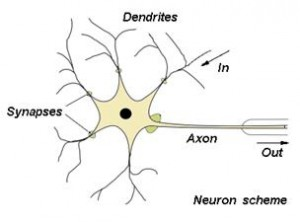
\includegraphics[scale=0.7]{figures/Chapter6AnnisaFathoroni2.jpg}
\caption{Konsep Dasar Neural Network - Annisa Fathoroni}
\label{Konsep Dasar Neural Network - Annisa Fathoroni}
\end{figure}

\end{itemize}

\item Konsep pembobotan Neural Network, dilengkapi dengan ilustrasi atau gambar.

Bobot merupakan suatu nilai yang mendefinisikan tingkat atau kepentingan hubungan antara suatu node dengan node yang lain. Semakin besar bobot  suatu hubungan menandakan semakin pentingnya hubungan kedua node tersebut. Bobot merupakan suatu hubungan berupa bilangan real maupun integer, tergantung dari jenis permasalahan dan model yang digunakan. Bobot-bobot tersebut bisa ditentukan untuk berada didalam interval tertentu. selama proses pelatihan, bobot tersebut dapat menyesuaikan dengan pola-pola input.

\begin{itemize}
\item Ilustrasi Gambar :

\begin{figure}[!hbtp]
\centering
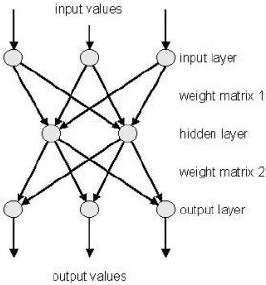
\includegraphics[scale=0.7]{figures/Chapter6AnnisaFathoroni3.jpg}
\caption{Konsep Pembobotan Neural Network - Annisa Fathoroni}
\label{Konsep Pembobotan Neural Network - Annisa Fathoroni}
\end{figure}

\end{itemize}

\item Konsep fungsi aktifasi dalam Neural Network, dilengkapi dengan ilustrasi atau gambar.
Operasi matematik yang dikenakan pada sinyal output y. Sehingga fungsi ini akan digunakan untuk pengaktifan dan juga penonaktifan neuron.
\begin{itemize}
\item Dalam konsep fungsi aktivasi Neuron Network terdapat beberapa jenis:
\begin{itemize}
\item Fungsi Undak Biner Hard Limit ( Menkonversi nilai masukan dari suatu variabel )
\item Fungsi Undak Biner Threshold ( Menggunakan nilai ambang 0 sebagai batas eksekusil )
\item Fungsi Bipolar Symetric Hard Limit ( Mempunyai keluaran bernilai 1 dan 0 )
\item Fungsi Bipolar Threshold ( Mempunyai keluaran bernilai 1, 0 atau -1 )

\item Ilustrasi Gambar:

\begin{figure}[!hbtp]
\centering
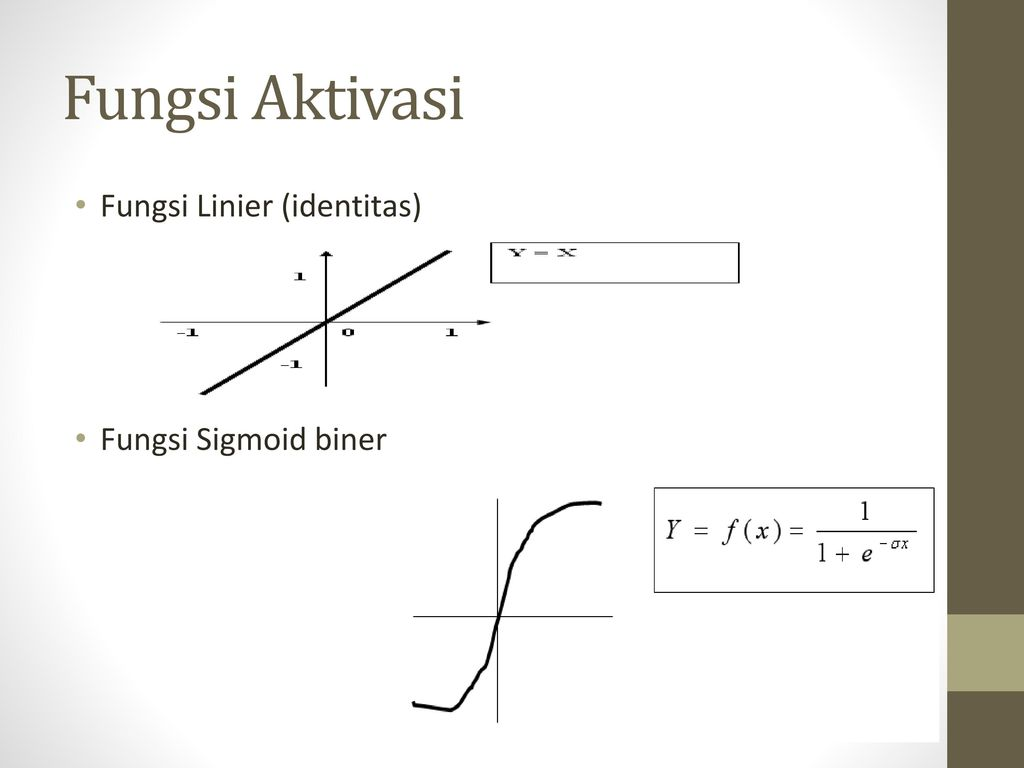
\includegraphics[scale=0.7]{figures/Chapter6AnnisaFathoroni4.jpg}
\caption{Konsep Fungsi Aktifasi - Annisa Fathoroni}
\label{Konsep Fungsi Aktivasi - Annisa Fathoroni}
\end{figure}

\end{itemize}
\end{itemize}

\item Cara membaca hasil plot dari MFCC, dilengkapi dengan ilustrasi atau gambar.

Penjelasan Cara Membaca Hasil Plot Dari MFCC :
\begin{itemize}
\item Ilustrasi Gambar :
\begin{figure}[!hbtp]
\centering
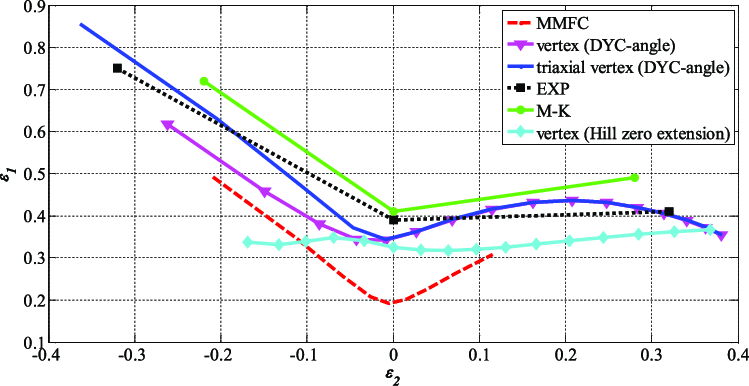
\includegraphics[scale=0.4]{figures/Chapter6AnnisaFathoroni5.png}
\caption{Plot MFCC - Annisa Fathoroni}
\label{Plot MFCC - Annisa Fathoroni}
\end{figure}

\end{itemize}

\item Apa itu One-Hot Encoding, dilengkapi dengan ilustrasi atau gambar.


One-Hot Encoding adalah sekelompok bit yang kombinasi hukumnya hanya terdiri dari bit dengan bit tinggi (1) dan bit lainnya rendah (0). Implementasi serupa di mana semua bit '1' kecuali satu '0' kadang-kadang disebut one-cold. Dalam statistik, variabel dummy mewakili teknik serupa untuk mewakili data kategorikal.
\begin{itemize}
\item Ilustrasi Gambar:

\begin{figure}[!hbtp]
\centering
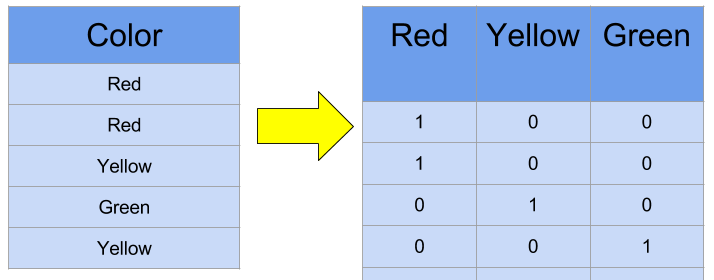
\includegraphics[scale=0.4]{figures/Chapter6AnnisaFathoroni6.png}
\caption{One-Hot Encoding - Annisa Fathoroni}
\label{One-Hot Encoding - Annisa Fathoroni}
\end{figure}

\end{itemize}

\item Fungsi dari np.unique dan to.categorical, dilengkapi dengan ilustrasi atau gambar.
\begin{enumerate}
\item np.unique:

Berfungsi untuk menemukan elemen unik array. Ada tiga output opsional selain elemen unik:

\begin{itemize}
\item Indeks array input yang memberikan nilai unik
\item Indeks array unik yang merekonstruksi array input
\item Berapa kali setiap nilai unik muncul dalam array input
\end{itemize}

\item Ilustrasi Gambar :

\begin{figure}[!hbtp]
\centering
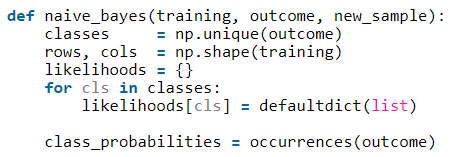
\includegraphics[scale=0.7]{figures/Chapter6AnnisaFathoroni7-1.png}
\caption{np.unique - Annisa Fathoroni}
\label{np.unique - Annisa Fathoroni}
\end{figure}

\item to.categorical:

Berfungsi untuk mengubah vektor kelas yang berupa integer menjadi matriks kelas biner.

\begin{itemize}
\item Ilustrasi Gambar :

\begin{figure}[!hbtp]
\centering
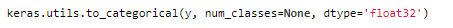
\includegraphics[scale=0.7]{figures/Chapter6AnnisaFathoroni7-2.png}
\caption{to.categorical - Annisa Fathoroni}
\label{to.categorical - Annisa Fathoroni}
\end{figure}

\end{itemize}
\end{enumerate}

\item Fungsi dari Sequential, dilengkapi dengan ilustrasi atau gambar.
Sebuah jenis model yang digunakan dalam perhitungan ataupun code program yang direalisasikan.
\begin{itemize}
\item Ilustrasi Gambar:

\begin{figure}[!hbtp]
\centering
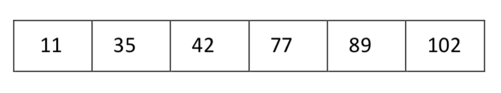
\includegraphics[scale=0.7]{figures/Chapter6AnnisaFathoroni8.png}
\caption{Sequential - Annisa Fathoroni}
\label{Sequential - Annisa Fathoroni}
\end{figure}

\end{itemize}
\end{enumerate}

\section{Tasya Wiendhyra / 1164086}
\subsection{Teori}
\begin{enumerate}
\item Kenapa file suara harus di lakukan MFCC. dilengkapi dengan ilustrasi atau gambar. \\
\par Nilai-nilai MFCC meniru pendengaran manusia dan mereka biasanya digunakan dalam aplikasi pengenalan suara serta genre musik
deteksi. Nilai-nilai MFCC ini akan dimasukkan langsung ke jaringan saraf.Agar dapat diubah menjadi bentuk vektor, dan dapat digunakan pada machine learning. Disebabkan machine learning hanya mengerti bilangan vektor saja.\\
Ilustrasinya, Ketika ingin menggunakan file suara dalam machine learning, misalnya untuk melihat jam. Machine learning tidak memahami rekaman suara melainkan vektor. Maka rekaman tersebut akan diubah kedalam bentuk vektor kemudian vektor akan menyesuaikan dengan kata kata yang sudah disediakan. Jika cocok maka akan mengembalikan waktu yang diinginkan

\item Konsep dasar neural network dilengkapi dengan ilustrasi atau gambar
\par Neural Network ini terinspirasi dari jaringan saraf otak manusia. Dimana setiap neuron terhubung ke setiap neuron di lapisan berikutnya. Lapisan pertama menerima input dan lapisan terakhir memberikan keluaran. Struktur jaringan, yang berarti jumlah neuron dan koneksinya, diputuskan sebelumnya dan tidak dapat berubah, setidaknya tidak selama training. Juga, setiap input harus memiliki jumlah nilai yang sama. Ini berarti bahwa gambar, misalnya, mungkin perlu diubah ukurannya agar sesuai dengan jumlah neuron input.\\

Ilustrasinya. misalkan kita ingin encode sebuah kalimat yaitu "what time is it" kemudian Anda menginisialisasi lapisan jaringan Anda dan hidden statel. Bentuk dan dimensi hidden state akan tergantung pada bentuk dan dimensi jaringan saraf berulang Anda. Kemudian Anda mengulangi input Anda, meneruskan kata danhidden state ke NN. NN mengembalikan output dan kondisi tersembunyi yang dimodifikasi. Anda terus mengulang sampai Anda kehabisan kata-kata. Terakhir Anda melewatkan output ke layer feedforward, dan itu mengembalikan prediksi. Bahwa kita ingin mengetahui pukul berapa sekarang.

\item Konsep pembobotan dalam neural network.dilengkapi dengan ilustrasi atau gambar
\par Bobot mewakili kekuatan koneksi antar unit. Jika bobot dari node 1 ke node 2 memiliki besaran lebih besar, itu berarti bahwa neuron 1 memiliki pengaruh lebih besar terhadap neuron. 2. Bobot penting untuk nilai input. Bobot mendekati nol berarti mengubah input ini tidak akan mengubah output. Bobot negatif berarti meningkatkan input ini akan mengurangi output. Bobot menentukan seberapa besar pengaruh input terhadap output. Seperti contoh berikut :
\begin{figure}[ht]
\centering
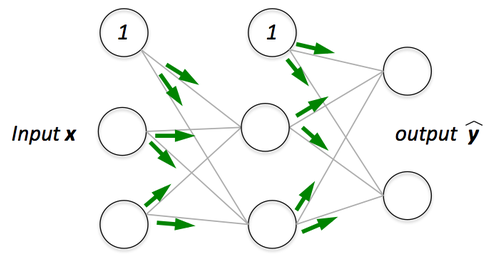
\includegraphics[scale=0.5]{figures/chapter6tasya2.png}
\caption{Contoh Pembobotan Neural Network Tasya}
\label{Teori}
\end{figure}

\item Konsep fungsi aktifasi dalam neural network. dilengkapi dengan ilustrasi atau gambar
\par Fungsi aktivasi digunakan untuk memperkenalkan non-linearitas ke jaringan saraf. Ini menekan nilai dalam rentang yang lebih kecil yaitu. fungsi aktivasi Sigmoid memeras nilai antara rentang 0 hingga 1. Ada banyak fungsi aktivasi yang digunakan dalam industri pembelajaran yang dalam dan ReLU, SeLU dan TanH lebih disukai daripada fungsi aktivasi sigmoid. Ilustrasinya, ketika fungsi aktivasi linier, jaringan saraf dua lapis mampu mendekati hampir semua fungsi. Namun, jika fungsi aktivasi identik dengan fungsi aktivasi F (X) = X), properti ini tidak puas, dan jika MLP menggunakan fungsi aktivasi yang sama, seluruh jaringan setara dengan jaringan saraf lapis tunggal.

\item Cara membaca hasil plot dari MFCC,dilengkapi dengan ilustrasi atau gambar\\
Berikut merupakan hasil plot dari rekaman suara :
\begin{figure}[ht]
\centering
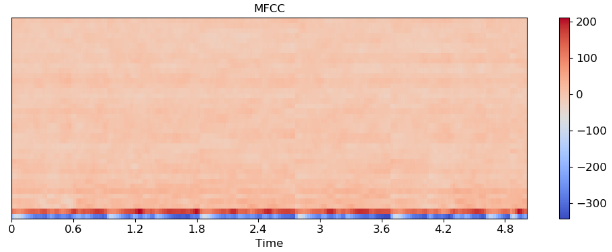
\includegraphics[scale=0.5]{figures/chapter6tasya1.png}
\caption{Cara Membaca Hasil Plot MFCC Tasya}
\label{Teori}
\end{figure}
Dari gambar tersebut dapat diketahui :\\
\begin{itemize}
\item Terdapat 2 dimensi yaitu x sebagai waktu, dan y sebagai power atau desibel.
\item Dapat dilihat bahwa jika berwarna biru maka power dari suara tersebut rendah, dan jika merah power dari suara tersebut tinggi
\item Dibagian atas terdapat warna merah pudar yang menandakan bahwa tidak ada suara sama sekali dalam jangkauan tersebut.
\end{itemize}

\item Jelaskan apa itu one-hot encoding,dilengkapi dengan ilustrasi kode dan atau gambar.
\par One-hot encoding adalah representasi variabel kategorikal sebagai vektor biner. Mengharuskan nilai kategorikal dipetakan ke nilai integer. Kemudian, setiap nilai integer direpresentasikan sebagai vektor biner yang semuanya bernilai nol kecuali indeks integer, yang ditandai dengan 1.
\begin{figure}[ht]
\centering
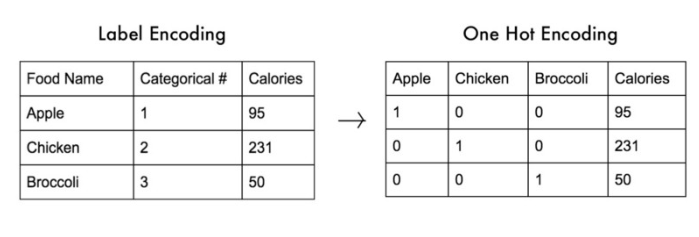
\includegraphics[scale=0.5]{figures/chapter6tasya3.png}
\caption{One Hot Encoding Tasya}
\label{Teori}
\end{figure}

\item fungsi dari np/.unique dan to categorical dalam kode program,dilengkapi dengan ilustrasi atau gambar.\\
Untuk np unique fungsinya yaitu menemukan elemen unik array. Mengembalikan elemen unik array yang diurutkan. Ada tiga output opsional selain elemen unik:\\
\begin{itemize}
\item Indeks array input yang memberikan nilai unik
\item Indeks array unik yang merekonstruksi array input
\item Berapa kali setiap nilai unik muncul dalam array input.
\end{itemize}
\begin{figure}[ht]
\centering
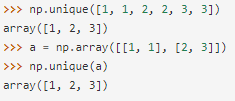
\includegraphics[scale=0.5]{figures/chapter6tasya4.png}
\caption{Numpy Unique Tasya}
\label{Teori}
\end{figure}

Untuk  To Categorical fungsinya untuk mengubah vektor kelas (integer) ke matriks kelas biner.
\begin{figure}[ht]
\centering
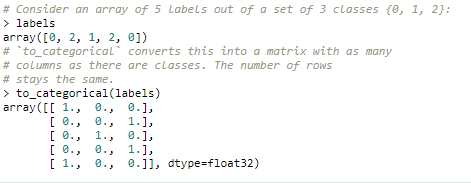
\includegraphics[scale=0.5]{figures/chapter6tasya5.png}
\caption{To Categorical Tasya}
\label{Teori}
\end{figure}

\item Fungsi dari Sequential dalam kode program,dilengkapi dengan ilustrasi atau gambar.\\
Sequential berfungsi sebagai tumpukan linear lapisan. COntohnya sebagai berikut :
\begin{figure}[ht]
\centering
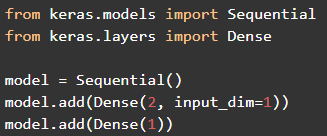
\includegraphics[scale=0.5]{figures/chapter6tasya6.png}
\caption{Sequential Tasya}
\label{Teori}
\end{figure}
\end{enumerate}

\section{Annisa Cahyani-1164066}
\subsection{Teori}
Penjelasan Tugas Harian11 ( No 1-8 )
\begin{enumerate}
\item Mengapa File Suara Harus Dilakukan MFCC Dilengkapi Dengan Ilustrasi Atau Gambar :
\par Yang Perlu kita ketahui disini yaitu  bahwa MFCC adalah Mel Frequency Cepstral Coefficients itu yang merupakan suatu koefisien yang merepresentasikan sebuah audio yang lebih simpel digunakan untuk sebagai library. 
\begin{itemize}
\item Penjelasan Mengenai  File Suara Harus Dilakukan MFCC : 
\par Yang harus kita ketahui itu pada saat ingin melakukan MFCC ini kepada sebuah objek suara agar suara itu tersebut dapat berubah atau dapat diubah ke dalam bentuk data matrix yang telah diekstraksi oleh MFCC.
\end{itemize}
\par
\par
\item Konsep Dasar Neural Network Dilengkapi Dengan Ilustrasi Atau Gambar :
\par Neural Network adalah paradigma pemrosesan suatu informasi yang terinspirasi oleh sistim sel syaraf biologi, sama seperti otak yang memproses suatu informasi. 
\begin{itemize}
\item Penjelasan Konsep Dasar Neural Network
\par Neural Network merupakan kategori ilmu Soft Computing. Neural Network sebenarnya mengadopsi dari kemampuan otak manusia yang mampu memberikan stimulasi atau rangsangan, melakukan proses, dan memberikan output. Output diperoleh dari variasi stimulasi dan proses yang terjadi di dalam otak manusia.
\par
\par
\item Konsep Fungsi Aktifasi Dalam Neural Network Dilengkapi Dengan Ilustrasi Atau Gambar :
\begin{itemize}
\item Penjelasan Konsep Fungsi Aktifasi Dalam Neural Network :
\par Operasi matematik yang dikenakan pada sinyal outputnya. Fungsi aktivasi, ini berfungsi untuk seperti sinapsis. 
\item Dalam Konsep Fungsi Aktivasi Neuron Network Terdapat Beberapa Jenis, Yaitu :
\begin{itemize}
\item Fungsi Undak Biner Hard Limit ini untuk menkonversi sebuah nilai masukan dari suatu variabel
\item Fungsi Undak Biner Threshold disini untuk menggunakan nilai yang ambang 0 untuk batas eksekusil
\item Fungsi Bipolar Threshold untuk mempunyai keluaran bernilai yaitu1, 0 atau -1 
\item Fungsi Bipolar  Symetric Hard Limit untuk mempunyai keluaran nilai yang  bernilai hanya 1 dan 0
\par
\par
\end{itemize}
\end{itemize}
\par
\par
\item Cara Membaca Hasil Plot Dari MFCC Dilengkapi Dengan Ilustrasi Atau Gambar :
\begin{itemize}
\item Penjelasan Cara Membaca Hasil Plot Dari MFCC berpatokan terhadap hasil dari contoh yang telah diterapkan, sebagai salah satu contoh penjelasan yaitu dengan melakukan perhitungan dalam pendefinisian pemrosesan sinyal suara yang dieksekusi. Tentunya inputan / proses tersebut dapat dikombinasikan dengan penerapam lainnya sehingga memberikan hasil plot yang sesuai dengan pengeksekusian awal.
\par
\par
\end{itemize}
\par
\par
\item Apa itu One-Hot Encoding Dilengkapi Dengan Ilustrasi Atau Gambar :
\begin{itemize}
\item Penjelasan One-Hot Encoding : 
\par  One-hot yaitu suatu sekelompok bit di antaranya kombinasi nilai yang sah hanyalah yang dengan bit tinggi yaitu 1 dan yang rendah yaitu 0. Implementasi serupa di mana semua bit '1' kecuali satu '0' kadang-kadang disebut one-cold.
\par
\par
\end{itemize}
\par
\par
\item Fungsi Dari Unp.Unique Beserta To.Categorical Dilengkapi Dengan Ilustrasi Atau Gambar :
\begin{enumerate}
\item Penjelasan Fungsi Dari Unp.Unique :
\par  Dari Unp.Unique ini disini berfungsi untuk menemukan suatu elemen yang unik pada array, serta mempunyai 3 hasil output opsional yang selain elemen unik yaitu :
\begin{itemize}
\item yang pertama yaitu memiliki indeks pada array input agar dapat menghasilkan nilai yang unik
\item yang kedua yaitu suatu indeks pada array unik untuk merekontruksi array
\item dan yang ketiga yaitu harus dapat beberapa kali agar setiap nilai unik yang keluar itu ada dalam array input
\end{itemize}
\par
\par
\item Penjelasan Fungsi Dari To.Categorical :
\par To.Categorical ini disini berfungsi untuk mengubah sebuah vektor yang ada pada kelas yang berupa integer atau sebuah number untuk menjadi matriks yang kelas biner.
\par
\par
\end{enumerate}
\par
\par
\item Fungsi Dari Sequential Dilengkapi Dengan Ilustrasi Atau Gambar :
\begin{itemize}
\item Penjelasan Fungsi Dari Sequential :
\par Sequential ini dsini berfungsi untuk pencarian linear yang merupakan metode pencarian yang paling sederhana. Dengan menggunakan prinsip data yang ada dibandingkan satu per satu secara berurutan dengan data yang dicari sampai data tersebut ditemukan atau tidak ditemukan
\par
\par
\end{itemize}
\end{itemize}
\end{enumerate}

\section{Annisa Fathoroni/1164067}
\subsection{Praktek}
\begin{enumerate}
\item Penjelasan isi data GTZAN Genre Collection dan data dari Freesound.

\par Code Yang Digunakan :
\begin{figure}[!hbtp]
\centering
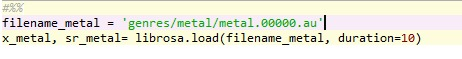
\includegraphics[scale=0.7]{figures/Chapter6AnnisaFathoroni16.jpeg}
\caption{Code GTZAN - Annisa Fathoroni}
\label{Code Display MFCC - Annisa Fathoroni}
\end{figure}

\begin{itemize}
\item Penjelasan isi data GTZAN:

\begin{enumerate}
\item Baris Code 1: Filename 'metal' merupakan variabel direktori dari file yang dituju, disini digunakan file audio dari genre 'metal'.
\item Baris Code 2: x metal dan sr metal variabel yang digunakan untuk meload file dari variabel filename metal menggunakan library librosa, yang nantinya akan digunakan pada MFCC.

\end{enumerate}

\item Ilustrasi Gambar:

\begin{figure}[!hbtp]
\centering
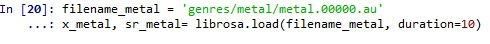
\includegraphics[scale=0.7]{figures/Chapter6AnnisaFathoroni17.jpeg}
\caption{GTZAN - Annisa Fathoroni}
\label{GTZAN - Annisa Fathoroni}
\end{figure}

\end{itemize}

\item Penjelasan perbaris kode program dari display MFCC.
\begin{itemize}
\item Code Yang Digunakan :
\begin{figure}[!hbtp]
\centering
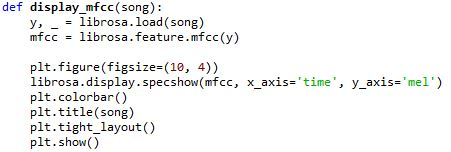
\includegraphics[scale=0.7]{figures/Chapter6AnnisaFathoroni14.jpg}
\caption{Code Display MFCC - Annisa Fathoroni}
\label{Code Display MFCC - Annisa Fathoroni}
\end{figure}

\item Penjelasan:

\begin{enumerate}
\item Baris Code 1: Membuat fungsi display MFCC untuk menampilkan vektorisasi dari sebuah suara dimana variabel parameter.
\item Baris Code 2: Membuat variabel Y dimana untuk membaca variable parameter song dari perintah librosa load.
\item Baris Code 3: Membuat variabel MFCC untuk memanggil variabel Y dan mengubah suara menjadi vektor.
\item Baris Code 4: Melakukan plotting gambar dengan ukuran 10x4 dari figsize.
\item Baris Code 5: Menampilkan spektogram dari library librosa dimana untuk x\_axis didefinisikan dengan time kemudian y\_axis di definisikan dengan mel.
\item Baris Code 6: Menambahkan colorbar pada plot yang dijalankan.
\item Baris Code 7: Menetapkan atau memberikan judul untuk suara yang dieksekusi.
\item Baris Code 8: Untuk menyesuaikan subplot params sehingga subplot cocok dengan area gambar.
\item Baris Code 9: Fungsi untuk menampilkan hasil plot dari inputan yang telah dieksekusi.
\end{enumerate}

\item Ilustrasi Gambar:

\begin{figure}[!hbtp]
\centering
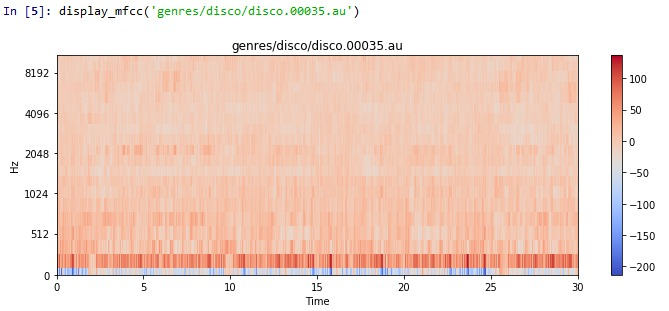
\includegraphics[scale=0.6]{figures/Chapter6AnnisaFathoroni11.jpeg}
\caption{Display MFCC - Annisa Fathoroni}
\label{Display MFCC - Annisa Fathoroni}
\end{figure}

\end{itemize}

\item Penjelasan perbaris code dari Extract Feature Song.
\begin{itemize}
\item Code yang digunakan:
\begin{figure}[!hbtp]
\centering
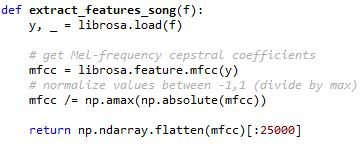
\includegraphics[scale=0.6]{figures/Chapter6AnnisaFathoroni15.jpg}
\caption{Code Extract Feature Song - Annisa Fathoroni}
\label{Code Extract Feature Song - Annisa Fathoroni}
\end{figure}
\item Penjelasan Code:
\begin{enumerate}
\item Baris Code 1 : Membuat fungsi extract feature song dengan inputan parameter f
\item Baris Code 2 : Membuat variabel y dimana untuk meload atau membaca inputan parameter f dari perintah librosa load song 
\item Baris Code 3 : Membuat variabel mfcc yang difungsikan untuk membuat feature dari variabel y berdasarkan library librosa
\item Baris Code 4 : Membuat normalisasi nilai antara -1 sampai 1 yang didapatkan dari eksekusi np.absolute
\item Baris Code 5 : Didefinisikan untuk mengambil 25000 data pertama berdasarkan durasi suara atau musik lalu dikembalikan salinan arraynya dan dikecilkan menjadi satu.
\end{enumerate}

\item Ilustrasi Gambar:

\begin{figure}[!hbtp]
\centering
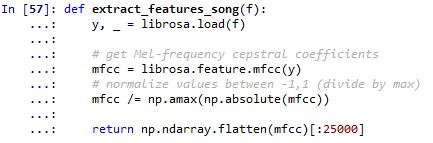
\includegraphics[scale=0.6]{figures/Chapter6AnnisaFathoroni12.jpg}
\caption{Extract Features Song - Annisa Fathoroni}
\label{Extract Features Song - Annisa Fathoroni}
\end{figure}

\item Mengapa yang diambil merupakan 25.000 baris data pertama?

Biar supaya tidak terjadi overhead pada komputer atau laptop atau proses eksekusi tidak terlalu lama.

\end{itemize}

\item Penjelasan perbaris code dari Generate Features and Labels.
\begin{itemize}
\item Penjelasan:
\begin{enumerate}
\item Baris Code 1: Membuat perintah untuk fungsi generate features and labels.
\item Baris Code 2: Pembuatan variabel all features dengan array atau parameter kosong.
\item Baris Code 3: Pembuatan variabel all labels dengan array atau parameter kosong.
\item Baris Code 4: Mendefinisikan variable genres yang didalamnya berisi nama folder-folder pada variabel genres tersebut.
\item Baris Code 5: Membuat perintah fungsi looping.
\item Baris Code 6: Membuat atribut sound files yang berisi perintah looping perfolder dari folder genres dan mengambil semua file berekstensi au.
\item Baris Code 7: Memunculkan jumlah song yang dieksekusi.
\item Baris Code 8: Membuat perintah fungsi dari sound files.
\item Baris Code 9: Membuat variabel features untuk memanggil fungsi extract features song (f) sebagai inputan. Setiap satu file array sound files dilakukan ekstrak fitur.
\item Baris Code 10: Memasukkan semua features menggunakan perintah append kedalam all features.
\item Baris Code 11: Memasukkan semua genres menggunakan perintah append ke dalam all labels.
\item Baris Code 12:Mendefinisikan label uniq ids dan label row ids sebagai variabel dimana mengeksekusi perintah np.unique dengan parameter variabelnya all labels dan return inverse=True.
\item Baris Code 13: Membuat variabel label row ids untuk menentukan type dari variabel tersebut dengan type bit yang sesuai dengan yang digunakan.
\item Baris Code 14: Membuat variabel onehot labels dimana mengeksekusi to categorical dengan variabel parameter low row ids dan len.
\item Baris Code 15: Mengembalikan dan menampilkan hasil eksekusi dari variabel parameter all features dan onehot labels perintah dari np.stack.
\end{enumerate}

\item Ilustrasi Gambar:

\begin{figure}[!hbtp]
\centering
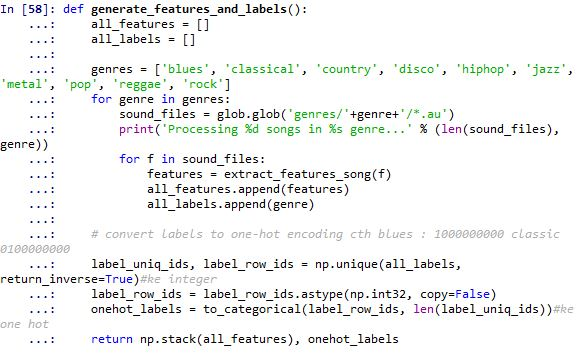
\includegraphics[scale=0.6]{figures/Chapter6AnnisaFathoroni13.jpg}
\caption{Generate Features and Label - Annisa Fathoroni}
\label{Generate Features and Label - Annisa Fathoroni}
\end{figure}

\end{itemize}

\item Penjelasan penggunaan fungsi Generate Features and Labels sangat lama ketika Meload Dataset Genre.
\begin{itemize}
\item Penjelasan:

Baris 1: Variabel features and label akn mengeksekusi isi dari features and label

Baris 2: Memproses 100 lagu di genre blues

Baris 3: Memproses 100 lagu di  genre classical

Baris 4: Memproses 100 lagu di  genre country

Baris 5: Memproses 100 lagu di  genre disco

Baris 6: Memproses 100 lagu di  genre  hip hop

Baris 7: Memproses 100 lagu di  genre jazz

Baris 8: Memproses 100 lagu di  genre metal

Baris 9: Memproses 100 lagu di genre pop

Baris 10: Memproses 100 lagu di genre reggae

Baris 11: Memproses 100 lagu di genre rock

\item Ilustrasi Gambar:

\begin{figure}[!hbtp]
\centering
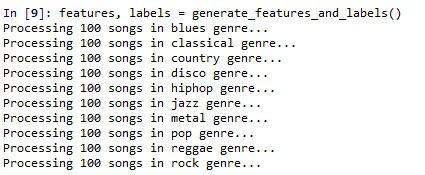
\includegraphics[scale=0.7]{figures/Chapter6AnnisaFathoroni18.jpg}
\caption{Fungsi Generate Features and Label Load Dataset Genre - Annisa Fathoroni}
\label{Fungsi Generate Features and Label Load Dataset Genre - Annisa Fathoroni}
\end{figure}

\end{itemize}

\end{enumerate}

\section{Annisa Cahyani-1164066}
\subsection{Praktek}
\begin{enumerate}
\item Penjelasan Mengenai Isi Data GTZAN Genre Collection Dan Data Dari Freesound.
\begin{itemize}
\item Penjelasan Isi Data GTZAN :
\par Pada GTZAN Genre Collection ini isinya itu seperti data musik yang telah di folderkan yang berdasarkan dengan genre lagu.
\par
\item Ilustrasi Gambar ( Contoh ) : \ref{cahya-chapter6-1}
\par
\begin{figure}[!hbtp]
\centering
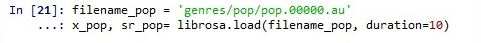
\includegraphics[scale=0.2]{figures/cahya-chapter6-1.jpg}
\caption{Contoh dari GTZA Genre Collection}
\label{cahya-chapter6-1}
\end{figure}
\par
\item Penjelasan Mengenai Contoh Code :
\begin{enumerate}
\item Baris Code yang pertama yaitu filename pop itu merupakan sebuah variabel yang berisikan direktori dari file yang ditujukan, dan code ini juga menggunakan file audio dari genre pop.
\item Baris Code yang kedua ini untuk membuat variabel x pop dan sr pop ini digunakan untuk meload file dari variabel filename pop yang menggunakan librari Librosa yang berdurasi 10.
\end{enumerate}
\end{itemize}
\par
\item Penjelasan Perbaris Kode Program Dari Display\_Mfcc.
\begin{itemize}
\item Penjelasan :
\par
\begin{enumerate}
\item Baris Code yang pertama itu kita membuat fungsi display pada mfcc untuk menampilkan sebuah vektorisasi dari song
\item Baris Code yang kedua itu membuat variabel Y untuk melakukan proses load atau untuk membaca sebuah variable. 
\item Baris Code yang ketiga yaitu membuat variabel mfcc yang berfungsi untuk memanggil variabel Y dan untuk mengubah song menjadi sebuah vektor
\item Baris Code yang keempat yaitu untuk melakuakan plotting sebuah gambar
\item Baris Code yang kelima yaitu berfungsi untuk menampilkan specshow dari library librosa
\item Baris Code yang keenam yaitu berfungsi untuk menambahkan sebuah colorbar
\item Baris Code yang ketujuh yaitu berfungsi untuk menetapkan judul untuk song yang akan dieksekusi
\item Baris Code yang kedelapan yaitu berfungsi untuk menyesuaikan tight layout sehingga tight layout itu cocok dengan gambar.
\item Baris Code yang kesembila yaitu berfungsi untuk menampilkan hasil dari show inputan
\end{enumerate}
\par
\item Ilustrasi Gambar : Ketika program tersebut dijalankan maka akan memberikan hasil seperti pada gambar berikut \ref {cahya-chapter6-2} dan \ref{cahya-chapter6-2-2}.
\par
\begin{figure}[!hbtp]
\centering
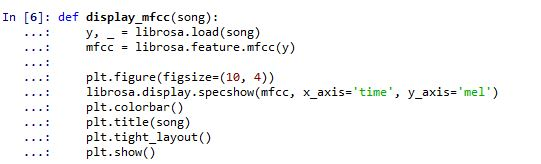
\includegraphics[scale=0.2]{figures/cahya-chapter6-2.jpg}
\caption{cahya-chapter6-2}
\label{cahya-chapter6-2}
\end{figure}
\par
\begin{figure}[!hbtp]
\centering
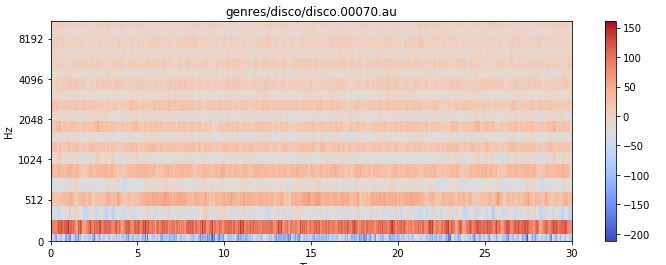
\includegraphics[scale=0.2]{figures/cahya-chapter6-2-2.jpg}
\caption{Cahya-chapter6-2-2}
\label{cahya-chapter6-2-2}
\end{figure}
\par
\end{itemize}
\par
\par
\par
\par
\par
\item Penjelasan Perbaris Code Dari Extract\_Feature\_Song().
\begin{itemize}
\item Penjelasan Code :
\begin{enumerate}
\item Baris Code yang pertama yaitu berfungsi untuk membuat suatu fungsi extract feature song dengan menggunakan sebuah yaitu inputan parameter f
\item Baris Code yang kedua yaitu berfungsi untuk membuat variabel pada y yang dimana itu berfungsi untuk membaca inputan pada parameter f 
\item Baris Code yang ketiga yaitu berfungsi untuk membuat sebuah variabel mfcc yang dimana difungsikan untuk membuat sebuah feature dari variabel y
\item Baris Code yang keempat yaitu berfungsi untuk membuat sebuah normalisasi pada nilai dari -1 sampai 1 
\item Baris Code yang kelima yaitu berfungsi untuk return = mengembalikan atau dapat didefinisikan untuk mengambil 25000 data yang pertama.
\end{enumerate}
\par
\item Ilustrasi Gambar : Ketika program tersebut dijalankan maka akan memberikan hasil seperti pada gambar berikut \ref{cahya-chapter6-3}.
\par
\begin{figure}[!hbtp]
\centering
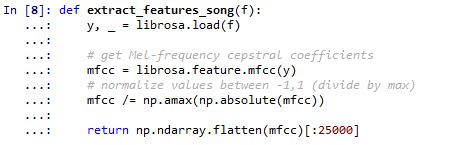
\includegraphics[scale=0.2]{figures/cahya-chapter6-3.jpg}
\caption{cahya-chapter6-3}
\label{cahya-chapter6-3}
\end{figure}
\par
\par
\item Mengapa Yang Diambil Itu Merupakan 25.000 Baris Data Pertama ?
\par Karena data yang digunakan itu hanya 25.000 dan pada baris data pertama sehingga dapat menghindari down pada sistem yang dieksekusi.
\par
\end{itemize}
\par
\par
\par
\par
\par
\par
\par
\item Penjelasan Perbaris Code Dari Generate\_Features\_And\_Labels().
\begin{itemize}
\item Penjelasan Code :
\begin{enumerate}
\item Baris Code yang pertama yaitu berfungsi untuk membuat sebuah perintah pada fungsi generate features and labels
\item Baris Code yang kedua yaitu berfungsi untuk pembuatan sebuah variabel all\_features dengan menggunakan parameter yang kosong
\item Baris Code yang ketiga yaitu berfungsi untuk pembuatan sebuah variabel all\_labels dengan menggunakan parameter yang kosong
\item Baris Code yang keempat yaitu berfungsi untuk membuat atau untuk mendefinisikan sebuah variable genres yang didalamnya berisikan nama folder-folder yang ada pada variabel genres tersebut.
\item Baris Code yang kelima yaitu berfungsi untuk membuat sebuah perintah pada fungsi looping
\item Baris Code yang keenam yaitu berfungsi untuk membuat sebuah atribut pada sound files yang dimana berisi perintah looping pada setiap folder dari folder yang genres dan mengambil semua file berekstensi au.
\item Baris Code yang ketujuh yaitu berfungsi untuk memunculkan song yang telah dieksekusi.
\item Baris Code yang kedelapan yaitu berfungsi untuk membuat sebuah perintah dari fungsi dari sound\_files
\item Baris Code yang kesembilan yaitu berfungsi untuk membuat sebuah variabel pada features untuk memanggil sebuah fungsi pada extract features song (f) itu sebagai inputan.
\item Baris Code yang kesepuluh yaitu berfungsi untuk memasukkan semua features yang menggunakan sebuah perintah append pada all\_features
\item Baris Code yang keseblas yaitu berfungsi untuk memasukkan semua genres yang telah menggunakan perintah append pada all\_labels
\item Baris Code yang keduabelas yaitu berfungsi untuk mendefinisikan sebuah label\_uniq\_ids dan label\_row\_ids itu sebagai variabel yang dimana akan mengeksekusi perintah np.unique
\item Baris Code yang ketigabelas yaitu berfungsi untuk membuat sebuah variabel label\_row\_ids untuk menentukan type yang ada pada variabel tersebut dengan menggunakan type bit yang sesuai yang digunakan.
\item Baris Code yang keempat belas yaitu berfungsi untuk membuat sebuah variabel onehot\_labels yang dimana akan mengeksekusi to\_categorical pada variabel yang parameter low\_row\_ids dan len(label\_uniq\_ids)
\item Baris Code yang kelima belas yaitu berfungsi untuk mengembalikan atau untuk menampilkan sebuah hasil eksekusi yang berasal dari variabel parameter all\_features dan onehot\_labels
\end{enumerate}
\par
\item Ilustrasi Gambar : Ketika program tersebut dijalankan maka akan memberikan hasil seperti pada gambar berikut \ref{cahya-chapter6-4}.
\par
\begin{figure}[!hbtp]
\centering
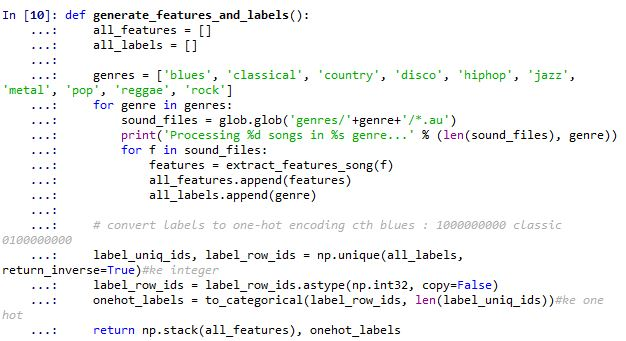
\includegraphics[scale=0.2]{figures/cahya-chapter6-4.jpg}
\caption{cahya-chapter6-4}
\label{cahya-chapter6-4}
\end{figure}
\par
\end{itemize}
\par
\par
\par
\par
\par
\par
\par
\par
\item Penjelasan Penggunaan Fungsi Generate\_Features\_And\_Labels() Sangat Lama Ketika Meload Dataset Genre.
\begin{itemize}
\par
\item Penjelasan : 
\par Disini fungsi pada Generate\_Features\_And\_Labels()ini akan sangat lama ketika meload sebuah dataset pada genre itu dikarenakan yang ada dalam dataset tersebut memilik 1000 data yang dimana pada 1000 data tersebut dibagi menjadi 10 bagian genre. 
\par
\item Ilustrasi Gambar : \ref{cahya-chapter6-5}
\par Penjelasan :
\par Dan hasil yang akan di dapatkan yaitu berada dari gambar yaitu dengan melakukan sebuah pemrosesan load untuk data pada masing genre. Yang dimana akan menghasilkan setiap genre itu terdiri dari 100 data yang apabila di akumulatifkan dengan 10 jenis genre musik.
\begin{figure}[!hbtp]
\centering
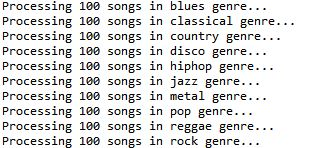
\includegraphics[scale=0.2]{figures/cahya-chapter6-5.jpg}
\caption{cahya-chapter6-5}
\label{cahya-chapter6-5}
\end{figure}
\par
\end{itemize}
\end{enumerate}
\par
\par
\par
\subsection{ Cahya - Penanganan Error Chapter 6}
\begin{enumerate}
\item Screenshoot Error : \ref{cahya-chapter6-error}
\par
\begin{figure}[!hbtp]
\centering
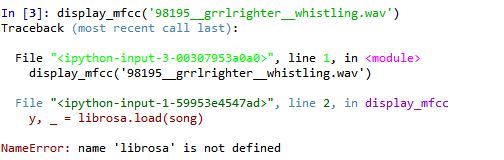
\includegraphics[scale=0.2]{figures/cahya-chapter6-error.jpg}
\caption{cahya-chapter6-error}
\label{cahya-chapter6-error}
\end{figure}
\par
\par
\item Code Error Yaitu :
\par Pada NameError: name 'librosa' is not defined
\item Penyelesaian Error :
\begin{enumerate}
\item Untuk menanganinya yaitu kita harus mendefinisikan library librosanya tersebut sebelum menjalankan perintahnya
\item Dan code yang harus dijalankan itu berfungsi untuk mendefinisikan library librosa
\par
\item Kemudia setelah itu silahkan jalankan code yang ada tersebut, kemudian jalankan kembali code yang telah menghasilkan error tadi
\item Apabila semua langkah-langkahnya telah diikuti maka tidak akan terjadi error lagi.
\end{enumerate}
\end{enumerate}
